\section{Virtual experiment}

For training and testing CLaNN we used synthetic data of biaxial stretching and inflation of a hyperelastic membrane, respectively.
% Synthetic experimental data description removed in English build
Model training was performed on numerical experimental data, 
obtained for biaxial stretching of a specimen with a "Maltese cross" geometry and thickness $H=0.53$ mm (Figure \ref{fig:malt_geometry}) using the hyperelastic nodal force method \cite{ddaniso2024}. 
The membrane material was specified by a neo-Hookean model \cite{ogden1997nonlinear}:
\begin{align} \label{eq:neohook}
        \widetilde{\psi} &= \dfrac{\mu H(X)}{2} (I_1 +J^{-2}-3),
        \quad     I_1 = e^{2\xi_1} (1+\xi_3^2)+e^{2\xi_2},\quad J = e^{\xi_1+\xi_2}
\end{align}
with $\mu=0.43\cdot 10^6$ Pa.

% Details of data extraction across specimen regions (omitted)
% Equilibrium method is described in \cite{ddaniso2024}.

\begin{figure}[H]
  \centering
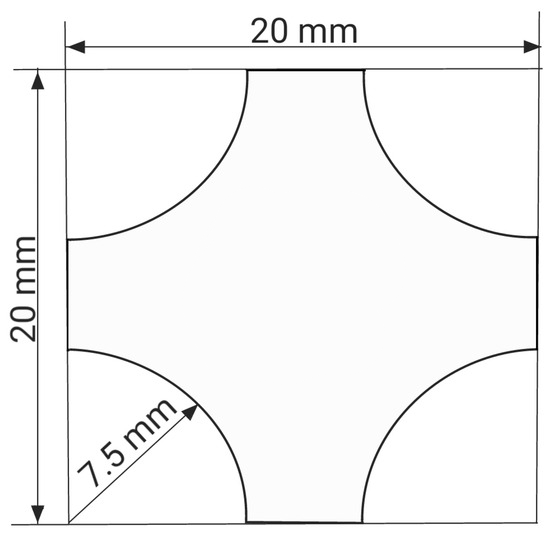
\includegraphics[width=0.4\textwidth]{../img/malt_geom.png}
\caption{Dimensions of the biomaterial specimen in the shape of a Maltese cross. 
  The cutout radius is the same for all notches}
  \label{fig:malt_geometry}
  \label{fig:malt_displacements}
\end{figure}

The specimen loading scheme is shown in Figure \ref{fig:malt_displacements}, where $w_i \in [0,1]$, $i \in \{1,4\}$
represents the fraction of the prescribed maximum displacement $u_{\max}$ for the $i$-th arm: $w_i = 0$ 
corresponds to a fixed arm, and $w_i = 1$ corresponds to the arm whose position was shifted and fixed at distance $u_{max}$. 
By varying $w_i$, different biaxial loading scenarios are obtained. 
In our virtual experiments we sequentially
displace the arms with increment $\Delta s$. 
The displacement $w_i \cdot n \cdot \Delta s$ is applied to the $i$-th arm at step $n$, where $n = 1, \ldots, N$, 
$N = u_{\max}/\Delta s$ is the number of steps. 
The hyperelastic nodal force method was applied to the initially flat quasi-uniform unstructured triangulation with mesh size $h=0.5$ mm and size $5\,404$ triangles. The maximum arm displacement
$u_{\max} = 2$ mm and $\Delta s = 0.2$ mm.
At each step, $\mathbb{C}, \mathbb{S}$ were extracted for all triangles belonging to the selected observation window. 
% Using linear (P1) elements, (C,S) are cellwise constants.

 
 
Our testing protocol comprises nine experiments:

\begin{figure}[H]
  \centering
  \begin{minipage}[t]{0.48\textwidth}
    \centering
    \vspace{0pt}
    \begin{tabular}{|c|c|c|c|c|}
    \hline
    \textbf{No.} & $w_1$ & $w_2$ & $w_3$ & $w_4$ \\
    \hline
    1 & 1 & 1 & 1 & 1 \\
    2 & 1 & 0.75 & 1 & 0.75 \\
    3 & 0.75 & 1 & 0.75 & 1 \\
    4 & 1 & 0.5 & 1 & 0.5 \\
    5 & 0.5 & 1 & 0.5 & 1 \\
    6 & 1 & 1/3 & 1 & 1/3 \\
    7 & 1/3 & 1 & 1/3 & 1 \\
    8 & 1 & 0 & 1& 0 \\
    9 & 0 & 1 & 0 & 1 \\
    \hline
    \end{tabular}
\captionof{table}{Test experiment protocols}
    \label{tab:test_protocols}
  \end{minipage}\hfill
  \begin{minipage}[t]{0.48\textwidth}
    \centering
    \vspace{0pt}
    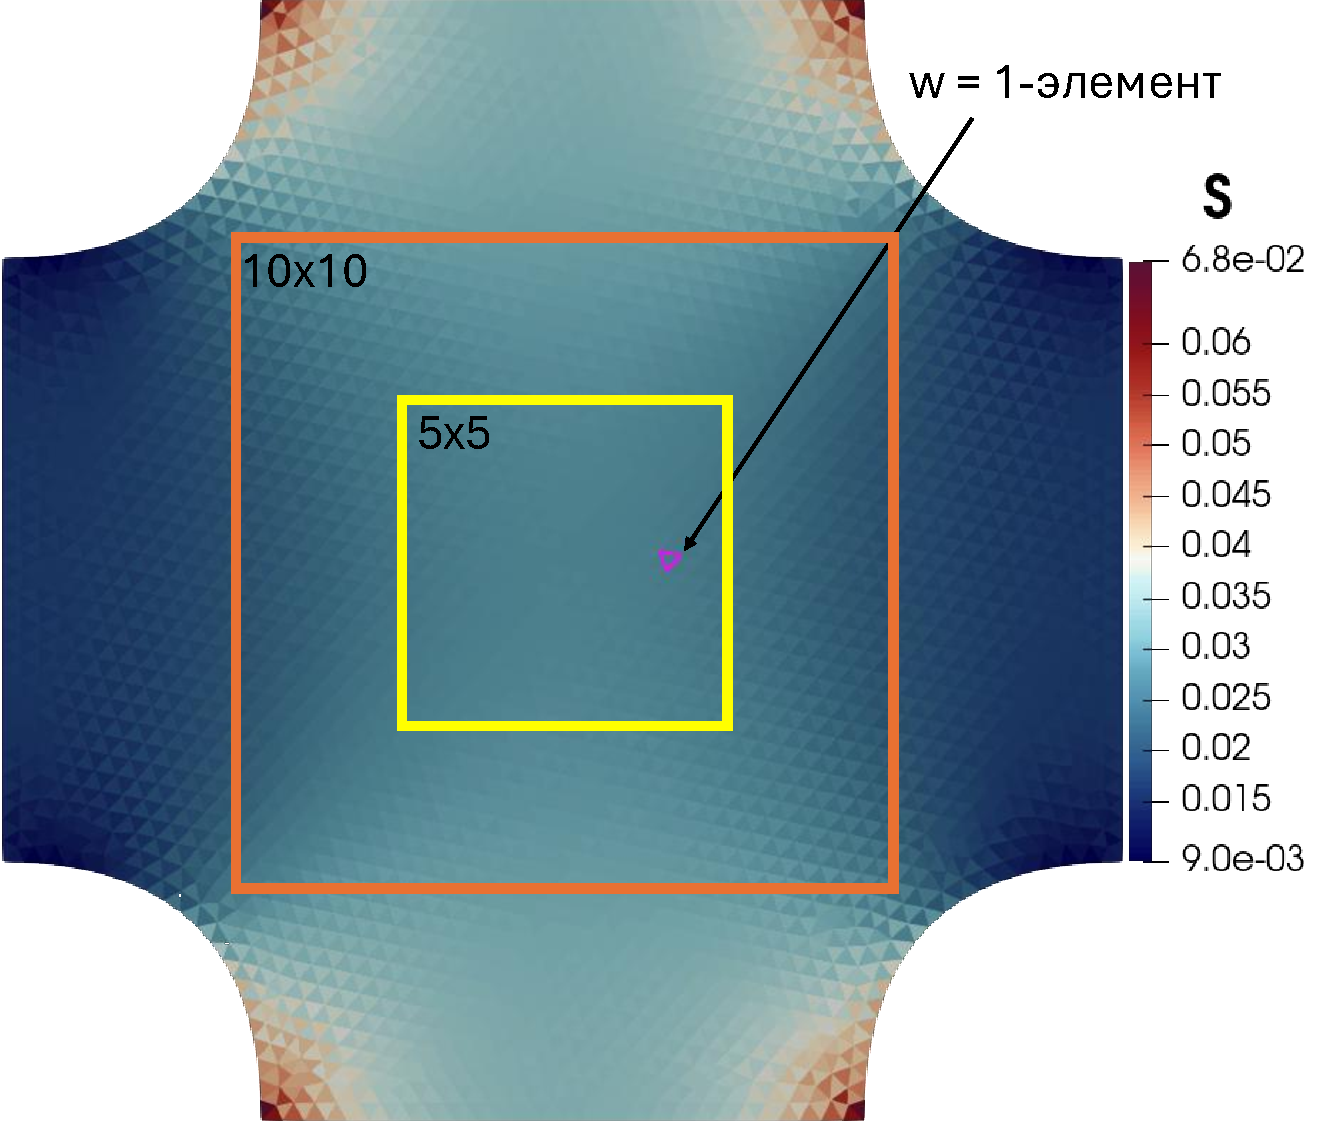
\includegraphics[width=\linewidth]{../img/Numerical/malt_window.pdf}
\captionof{figure}{Stress field $\vect S$ of the deformed membrane with "Maltese cross" geometry for different observation windows $w$.}
    \label{fig:malt_window}
  \end{minipage}
\end{figure}

\subsubsection{Data selection rules}
\paragraph{Central window $w$.}
The window is defined in the reference configuration $\Omega_0$ as the central region around the geometric center, aligned with the mesh axes. For $w=5\times5$ mm and $w=10\times10$ mm, we take squares of side 5 and 10 mm, respectively, centered at the specimen center; for $w=\text{full field}$ we take the entire $\Omega_0$. For $w=\text{1-element}$ we take the single central triangle (the minimal-index cell in the 5x5 mm window in $\Omega_0$ as shown in Figure~\ref{fig:malt_window}). Observations include all triangles whose barycenters $\mathbf{X}_T$ lie within the chosen window $\mathcal{W}_w\subset\Omega_0$.
% TODO: window cardinality in cells

\paragraph{Composition of observations (data).}
At each load step $n=1,\dots,N$ and for each triangle $T\in\mathcal{T}_w$ (cells within the window) we record the pair $(\mathbb C_T^{(n)},\,\mathbb S_T^{(n)})$, where $\mathbb C$ is the right Cauchy--Green tensor and $\mathbb S$ is the PK2 stress. Units: window sizes in mm; $\mathbb C$ dimensionless; $\mathbb S$ in MPa. Typical counts: 1 ($w=\text{1-element}$), 252 ($5\times5$ mm), 954 ($10\times10$ mm), and 5404 (full field).

\paragraph{Dataset formation.}
For fixed $(p,w)$, the set of all pairs $(\mathbb C_T^{(n)},\,\mathbb S_T^{(n)})$ forms the base dataset $D(p,w)$, which is split into $D_{\mathrm{tr}}(p,w)$ and $D_{\mathrm{val}}(p,w)$. For protocols $p$ (Table~\ref{tab:test_protocols}) and windows $w\in\{\text{1-element},5\times5\,\text{mm},10\times10\,\text{mm},\text{full field}\}$, denote
\[
  D_{\mathrm{tr}}\equiv D_{\mathrm{tr}}(p,w),\qquad D_{\mathrm{val}}\equiv D_{\mathrm{val}}(p,w),
\]
where $D_{\mathrm{tr}}$ is the training set and $D_{\mathrm{val}}$ is the validation set.

For example, $|D(\{1..10\}, \text{1-element})|=90$ points of $(\mathbb C,\mathbb S)$ (Figure \ref{fig:training_data}).

\begin{figure}[H]
  \centering
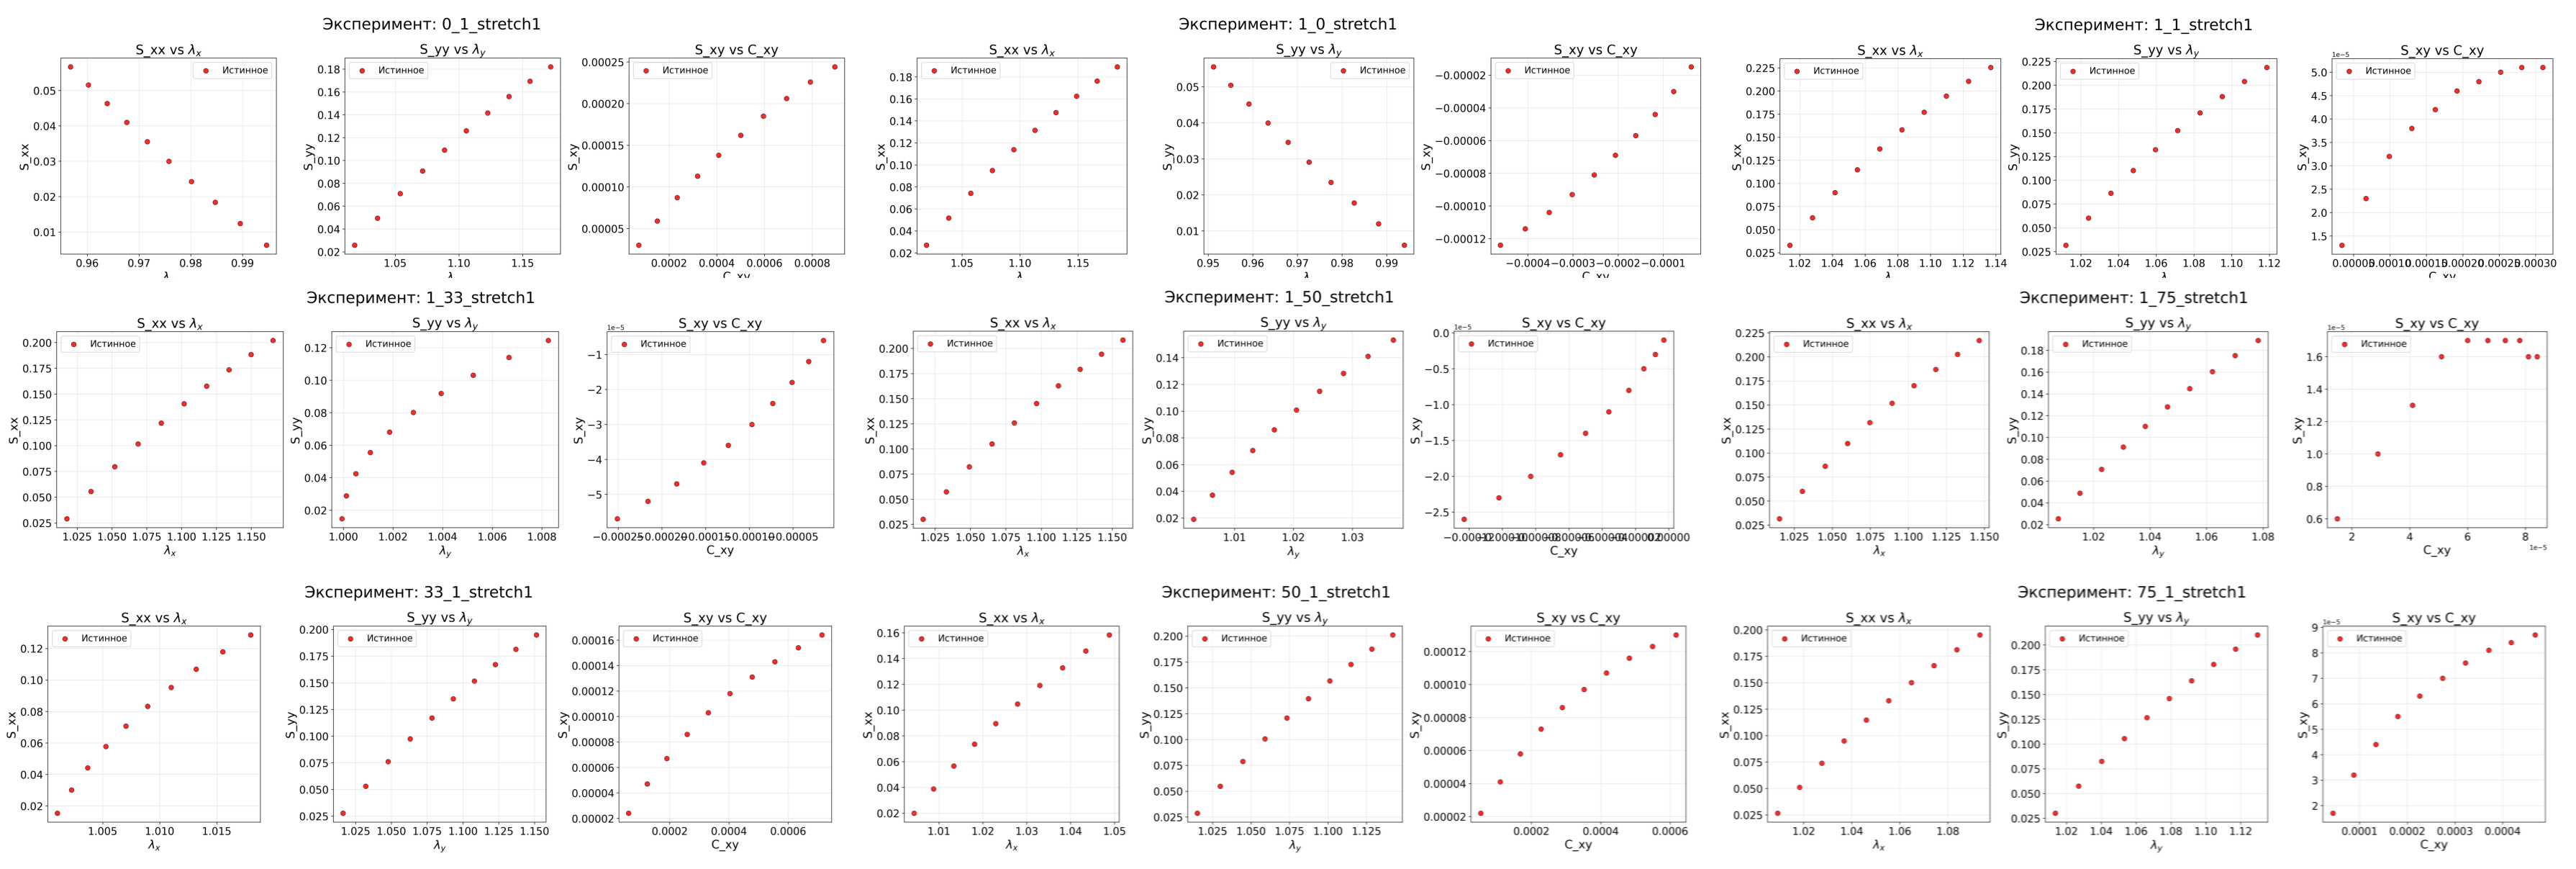
\includegraphics[width=1.0\textwidth]{../img/all_stress_plots.png}
\caption{Training dataset}
  \label{fig:training_data}
\end{figure}

Because data from a single central mesh element produce axial components much larger than shear ($2$--$3$ orders), expanding $w$ improves shear observability.

\subsubsection{Metrics and quality criteria}
\label{sec:metrics}

We use integral and pointwise metrics consistent with variational elasticity norms (e.g., \cite{ciarlet1988mathematical,ogden1997nonlinear,holzapfel2000nonlinear}).

\textbf{Coefficient of determination $R^2$.}
\begin{equation}\label{eq:r_squared}
  R^2 = 1 - \frac{\sum_{i=1}^n (y_i - \hat{y}_i)^2}{\sum_{i=1}^n (y_i - \bar{y})^2},
\end{equation}
where $y_i$ are experimental values, $\hat{y}_i$ are model predictions, $\bar{y}$ is the mean, and $n$ is the number of points.

\textbf{Pointwise relative error.}
\begin{equation}\label{eq:rel_error}
  \epsilon = \frac{\| \mathbb S - \mathbb S_{\text{ref}} \|}{\| \mathbb S_{\text{ref}} \|}.
\end{equation}
% purpose: plot error-field structure

\textbf{P1 error} \cite{xie2024p1} — a combination of absolute and relative errors, sensitive to small values:
\begin{equation}\label{eq:p1_error}
  \epsilon_{\mathrm{P1}} = \frac{\| \mathbb S - \mathbb S_{\text{ref}} \|}{s_0 + \| \mathbb S_{\text{ref}} \|},\qquad s_0 = \max(\mathbb S_{\text{pred}}).
\end{equation}

\textbf{Absolute integral error (mesh L2) for stresses (Frobenius norm).}
\begin{equation}\label{eq:l2_abs_stress}
  \|e\|_{L^2} = \Bigg( \sum_{K} \overline{\| \mathbb S_{\text{ref}} - \mathbb S_{\text{pred}} \|_F^{2}}^{\,K}\, |K| \Bigg)^{\tfrac12},
\end{equation}
where $|K|$ is the cell measure (area). For cell data, no intra-cell averaging is required:
\begin{equation}\label{eq:l2_abs_stress_cell}
  \|e\|_{L^2} = \Bigg( \sum_{K} \| \mathbb S_{\text{ref},K} - \mathbb S_{\text{pred},K} \|_F^{2}\, |K| \Bigg)^{\tfrac12}.
\end{equation}
Purpose: collapses the error field into a scalar and is invariant to mesh refinement \cite{BrennerScott2008,AinsworthOden2000,Verfurth2013}.

\textbf{Relative integral error.}
\begin{equation}\label{eq:l2_rel_stress}
  \|e\|_{L^2,\,\mathrm{rel}}\;=\; \frac{\Big( \sum\limits_{K} 
  \| \mathbb S_{\mathrm{ref},K} - \mathbb S_{\mathrm{pred},K} \|_F^{2}\, |K| \Big)^{\tfrac12}}
  {\Big( \sum\limits_{K} \| \mathbb S_{\mathrm{ref},K} \|_F^{2}\, |K| \Big)^{\tfrac12}}\,.
\end{equation}
% purpose: proper comparison across stress levels


\textbf{Optimization hyperparameters:}
\begin{itemize}
  \item Learning rate: $0.001$
  \item Batch size: $4$ (90-point set) and $128$ (other sets)
  % \item Physics weights: $\lambda_{\text{SI}} = 0.1$, $\lambda_{\psi} = 0.1$
  \item Architecture: 16 hidden neurons
  \item Smoothing parameter $\beta$: $10$
\end{itemize}

\textbf{Training results:}
Optimization reduces loss by five orders within $<5000$ epochs (Figure~\ref{fig:loss_curve}), reflecting both architectural suitability and hyperparameter choice; strict convexity ensures a unique minimum and avoids local traps.

\begin{figure}[H]
  \centering
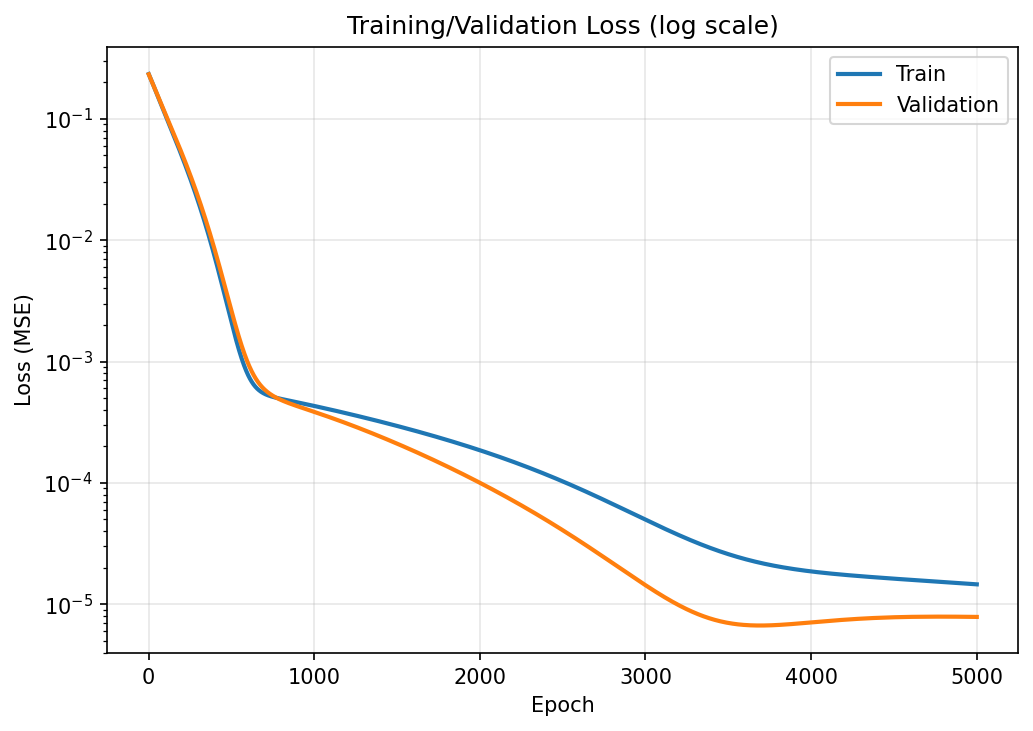
\includegraphics[width=0.7\textwidth]{../img/loss_curve.png}
  \caption{Loss curve when training on 90 data points}
  \label{fig:loss_curve}
\end{figure}


\subsection{Interpolation and extrapolation of loading curves}
We evaluate on $D_{\mathrm{tr}}(p,w)$ and $D_{\mathrm{val}}(p,w)$ at fixed $w$. We track $R^2_{\alpha}$, $\alpha\in\{xx,yy,xy\}$.

\textbf{Interpolation.}
Using 10 load levels from equi-biaxial ($p=1$), window $w=\text{1-element}$. CLANN achieves $R^2_{xx}=0.999$, $R^2_{yy}=0.999$, while $R^2_{xy}=0$ (Figure \ref{fig:interpolation}).

  \begin{figure}[H]
    \centering
    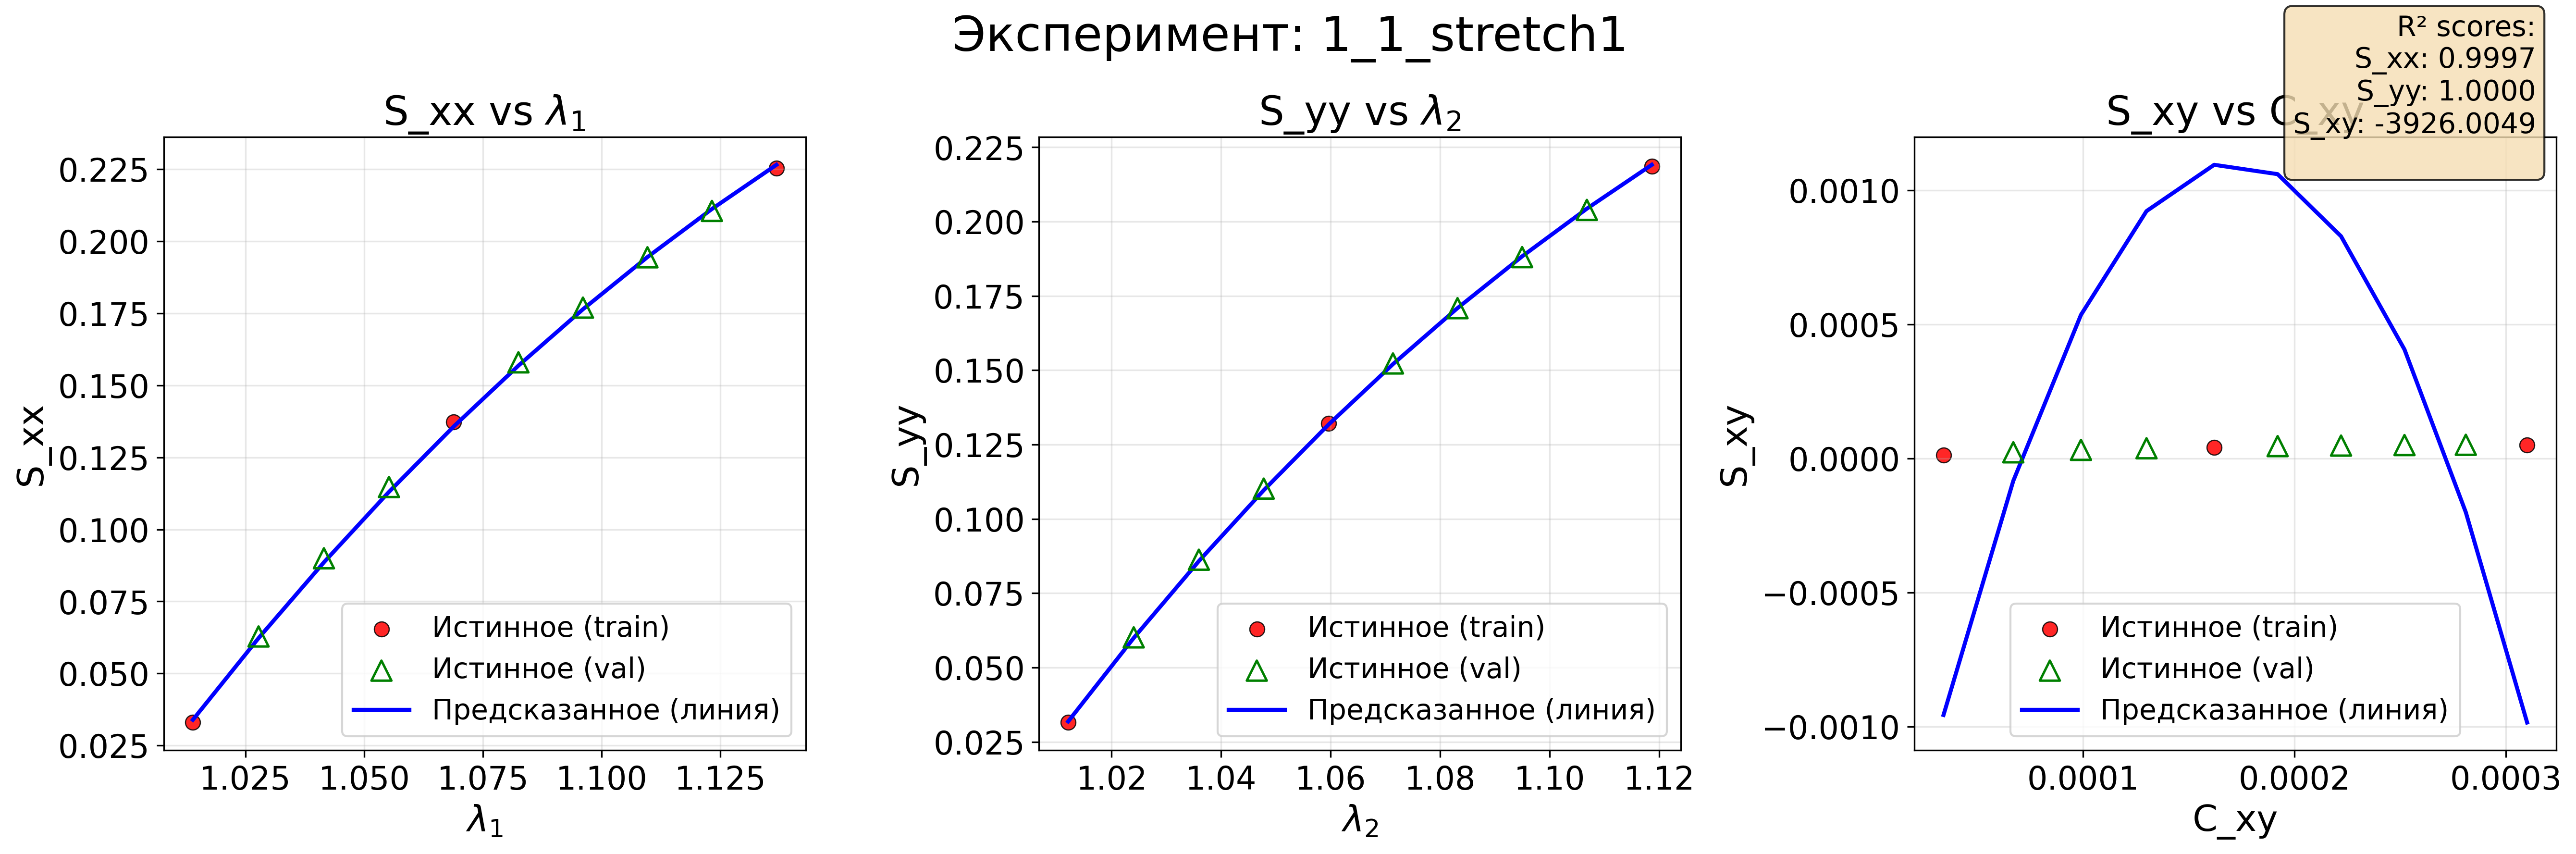
\includegraphics[width=1.0\textwidth]{../img/interpolation.png}
    \caption{Loading curve for equi-biaxial stretching}
    \label{fig:interpolation}
  \end{figure}
  
  \textbf{Extrapolation.}
  Train on $p=1$, validate on $p=9$, window $w=\text{1-element}$: $R^2_{xx}=0.993$, $R^2_{yy}=1.0$, $R^2_{xy}=0$ (Figure \ref{fig:extrapolation}).

  \begin{figure}[H]
    \centering
    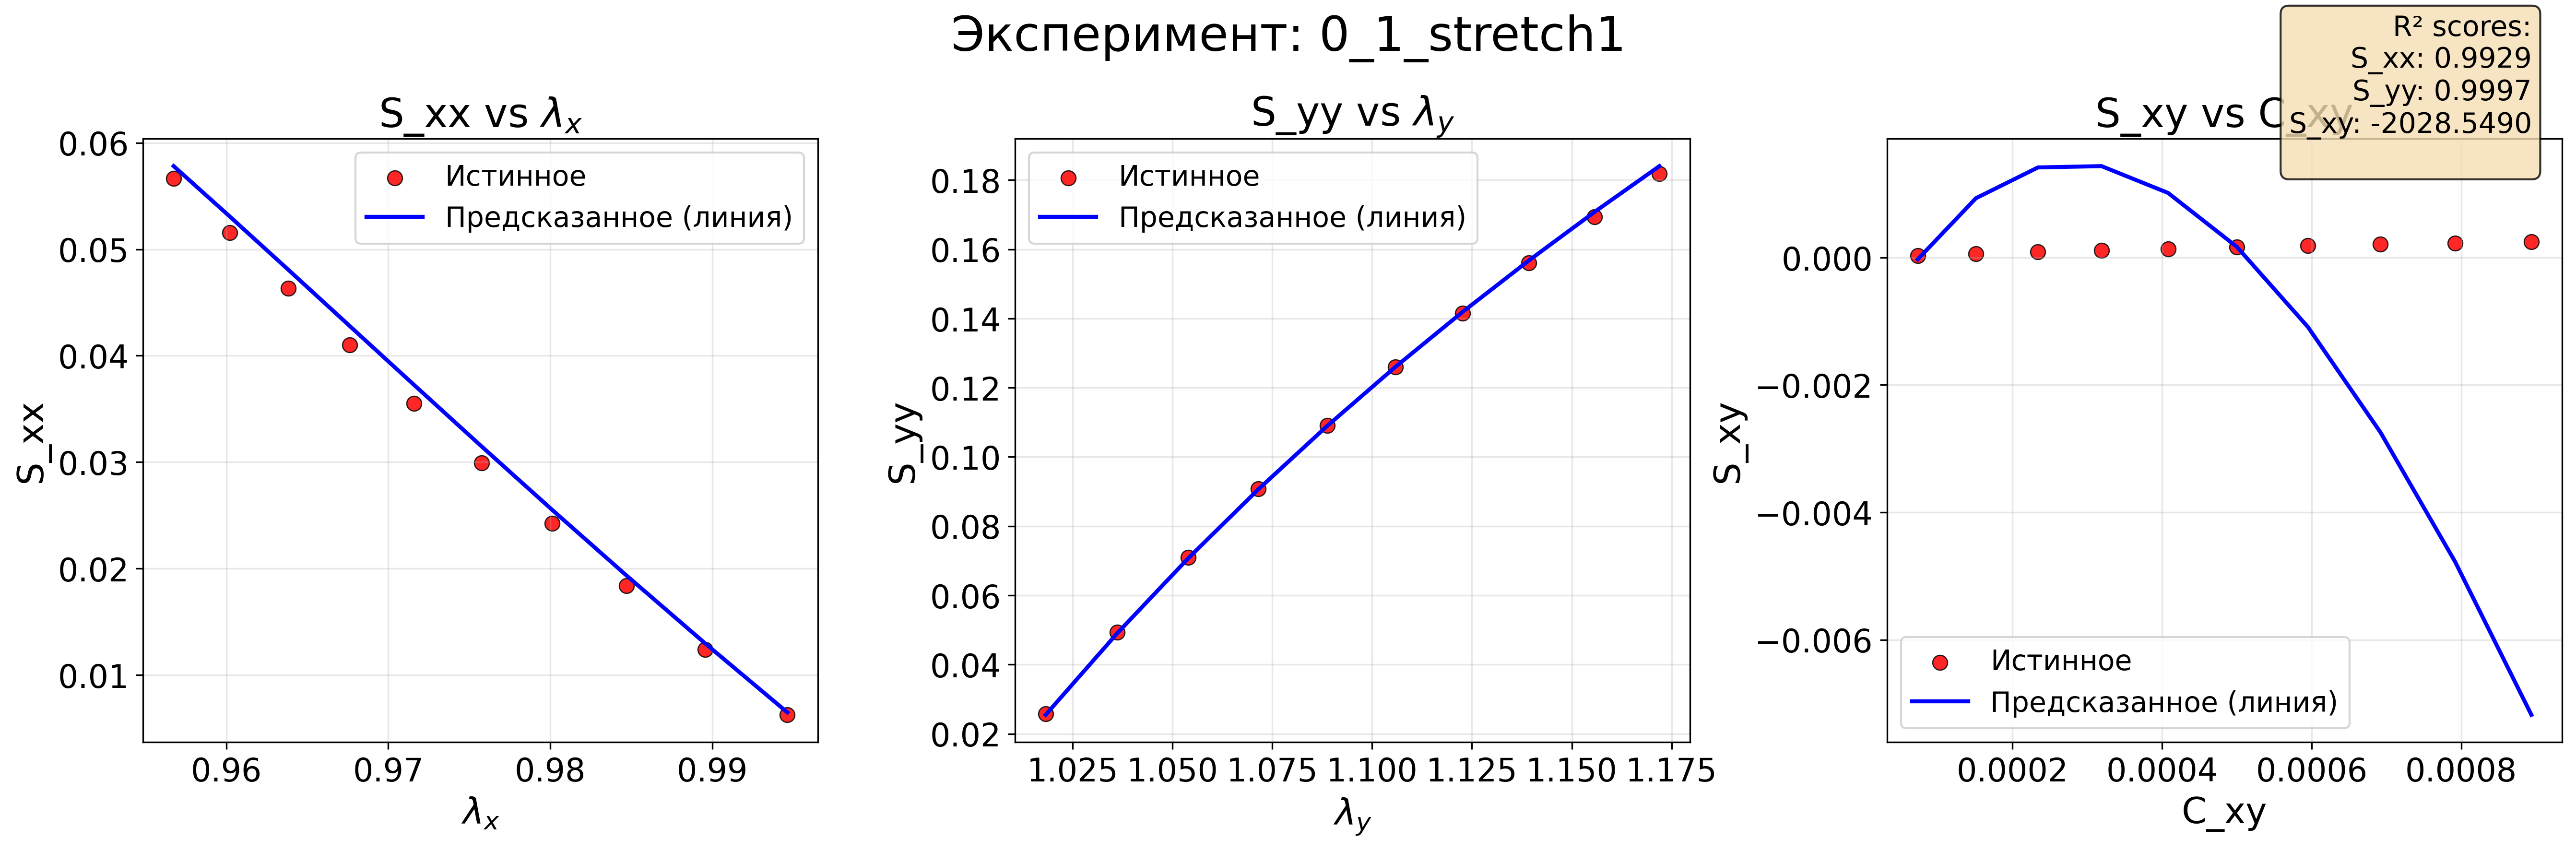
\includegraphics[width=1.0\textwidth]{../img/extrapolation.png}
    \caption{Loading curve for non-equi-biaxial stretching}
    \label{fig:extrapolation}
  \end{figure}
   
  Thus, CLANN interpolates and extrapolates axial components with high accuracy; shear prediction remains limited without richer shear coverage.
\subsection{Membrane inflation}

  We test inflation of a clamped circular membrane (radius 25 mm) under 5 MPa pressure, comparing CLANN to a Neo-Hookean reference with the same shear parameter as used in training-data generation.
  
  Two thickness fields $T$ are used: homogeneous (0.54 mm) and heterogeneous (two parabolic sectors of 2 mm within a 0.54 mm membrane), see Figure~\ref{fig:membrane_thickness}.

  As pointwise metric we use relative error (Section \ref{sec:metrics}, Eq.~\ref{eq:rel_error}); for shear comparison — P1 error \cite{xie2024p1} (Eq.~\ref{eq:p1_error}).

  \begin{figure}[H]
    \centering
    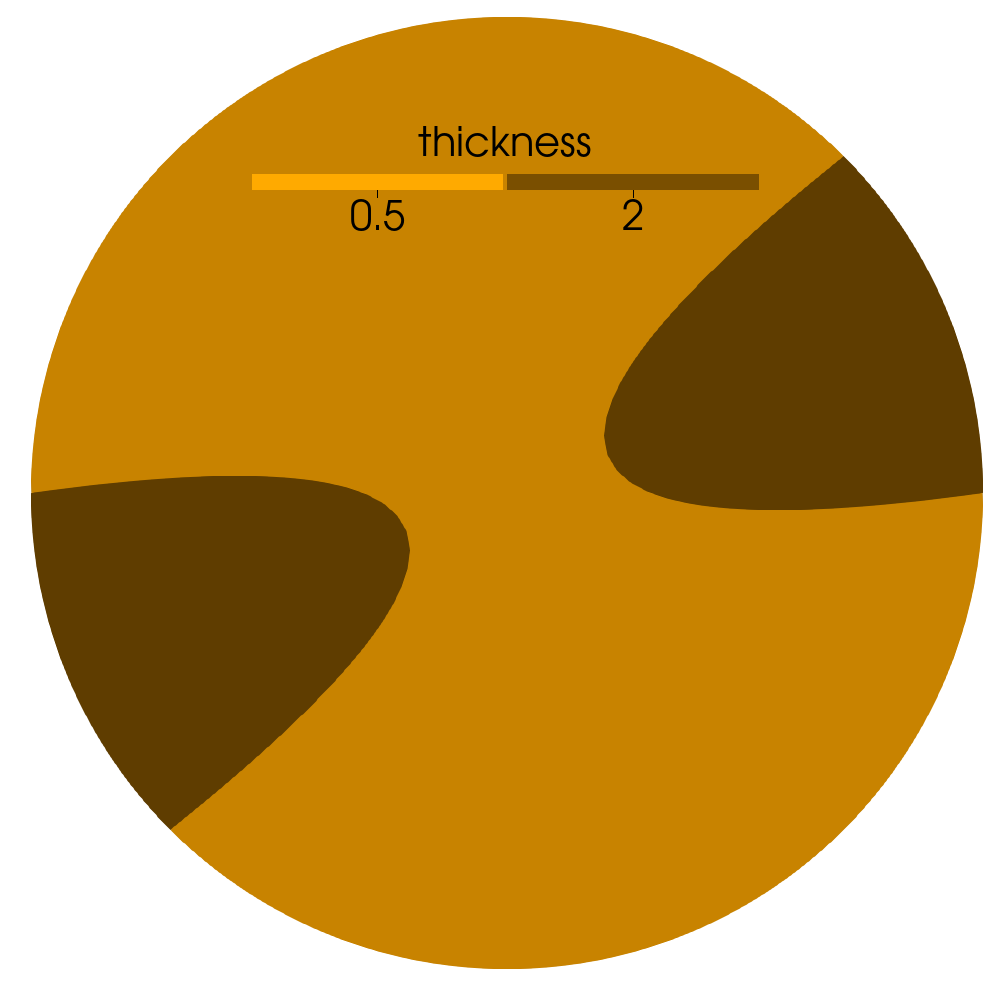
\includegraphics[width=0.25\linewidth]{../img/het_circle.png}
    \caption{Heterogeneous thickness field $T$ of the circular membrane.}
    \label{fig:membrane_thickness}
  \end{figure}

  \begin{figure}[H]
    \centering
    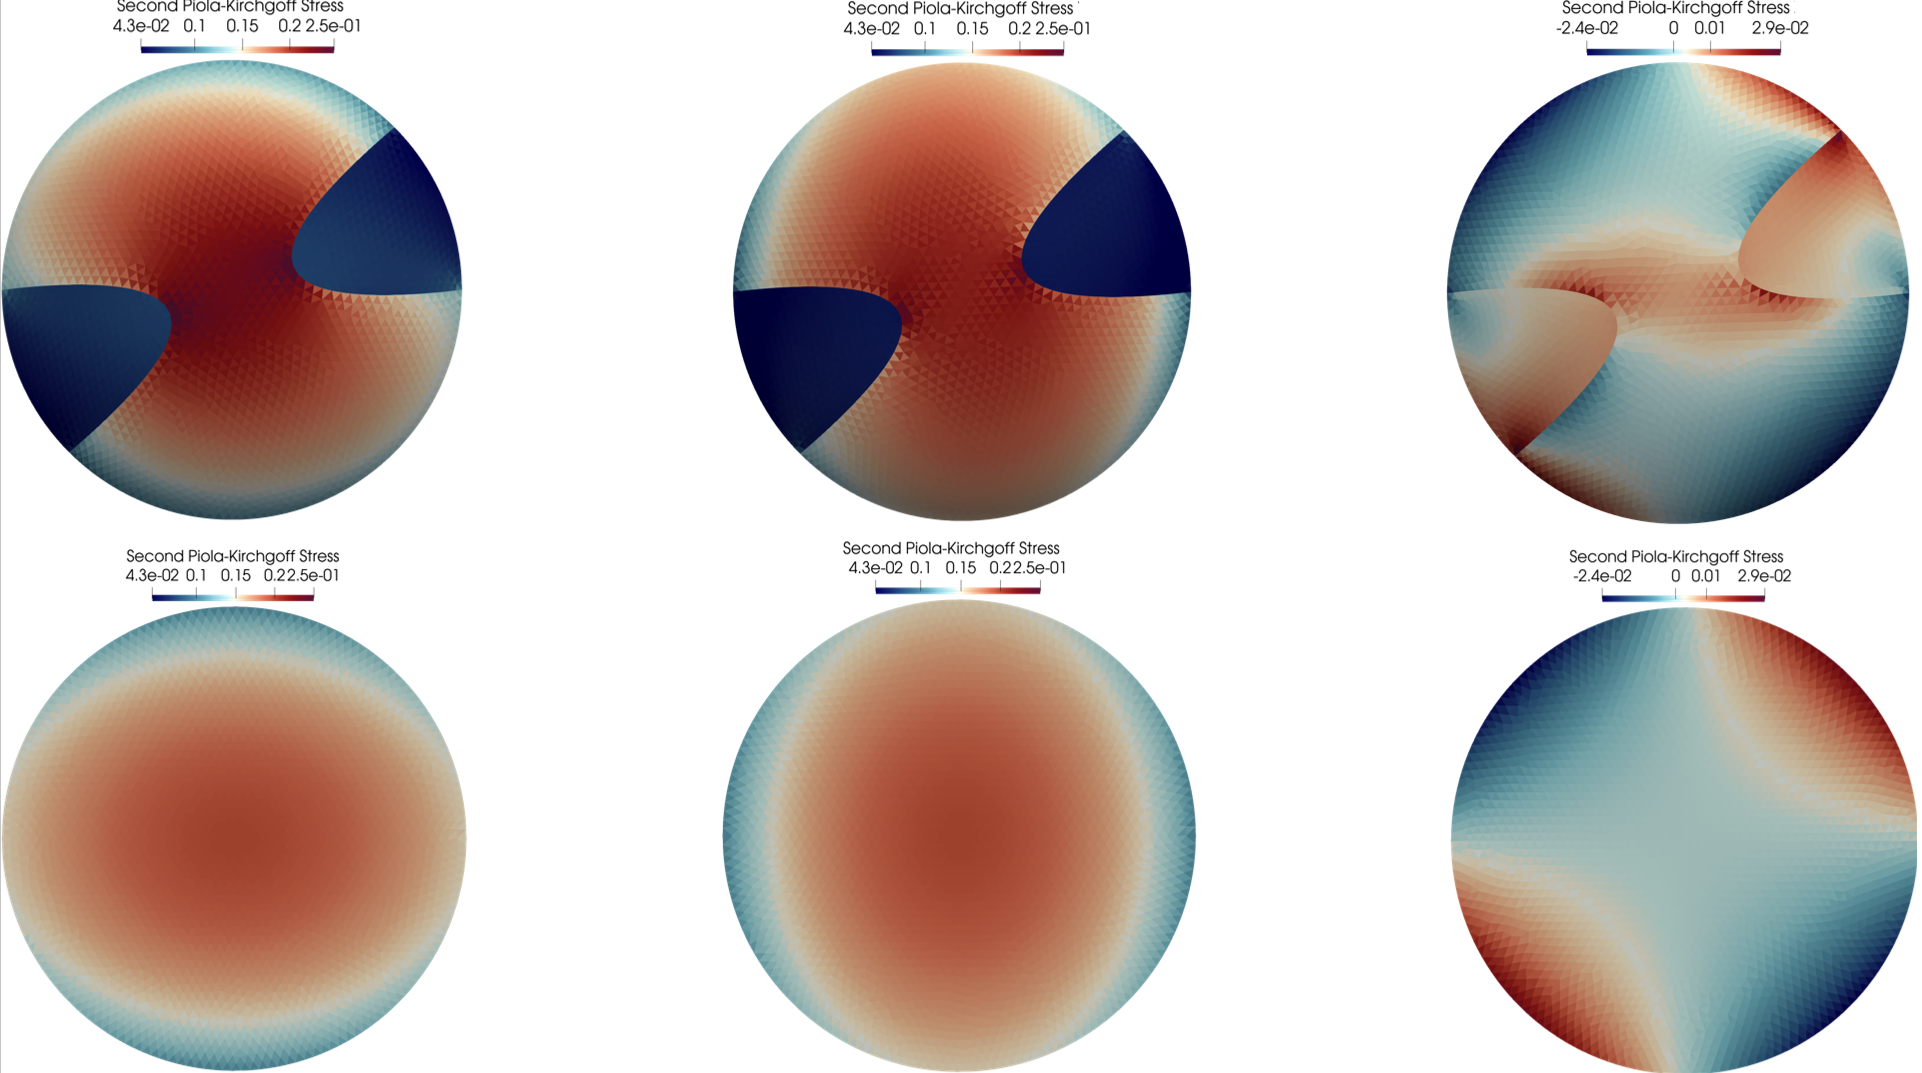
\includegraphics[width=0.7\textwidth]{../img/Numerical/ref_stress.png}
    \caption{PK2 stress field $\mathbb S$ of the circular membrane (example numerical result).}
    \label{fig:numerical_experiment}
  \end{figure}
  
  Using $D(\{1..10\}, w=\text{1-element})$ for training, we obtain PK2 stress fields for both thickness scenarios and compare to the reference (Figure~\ref{fig:membrane_thickness}, Figure~\ref{fig:inflation_ref}); error maps $\epsilon$ and $\epsilon_{P1}$ are shown in Figure~\ref{fig:numerical_errors}. Shear errors are largest for the heterogeneous case; expanding the window to $5\times 5$ mm, $10\times 10$ mm, and full field reduces integral errors $\|e\|_{L^2}$ (Eq.~\ref{eq:l2_abs_stress_cell}) and $\|e\|_{L^2,\,\mathrm{rel}}$ (Eq.~\ref{eq:l2_rel_stress}) (Figure~\ref{fig:integral_errors}).
  
  
  \begin{figure}[H]
    \centering
    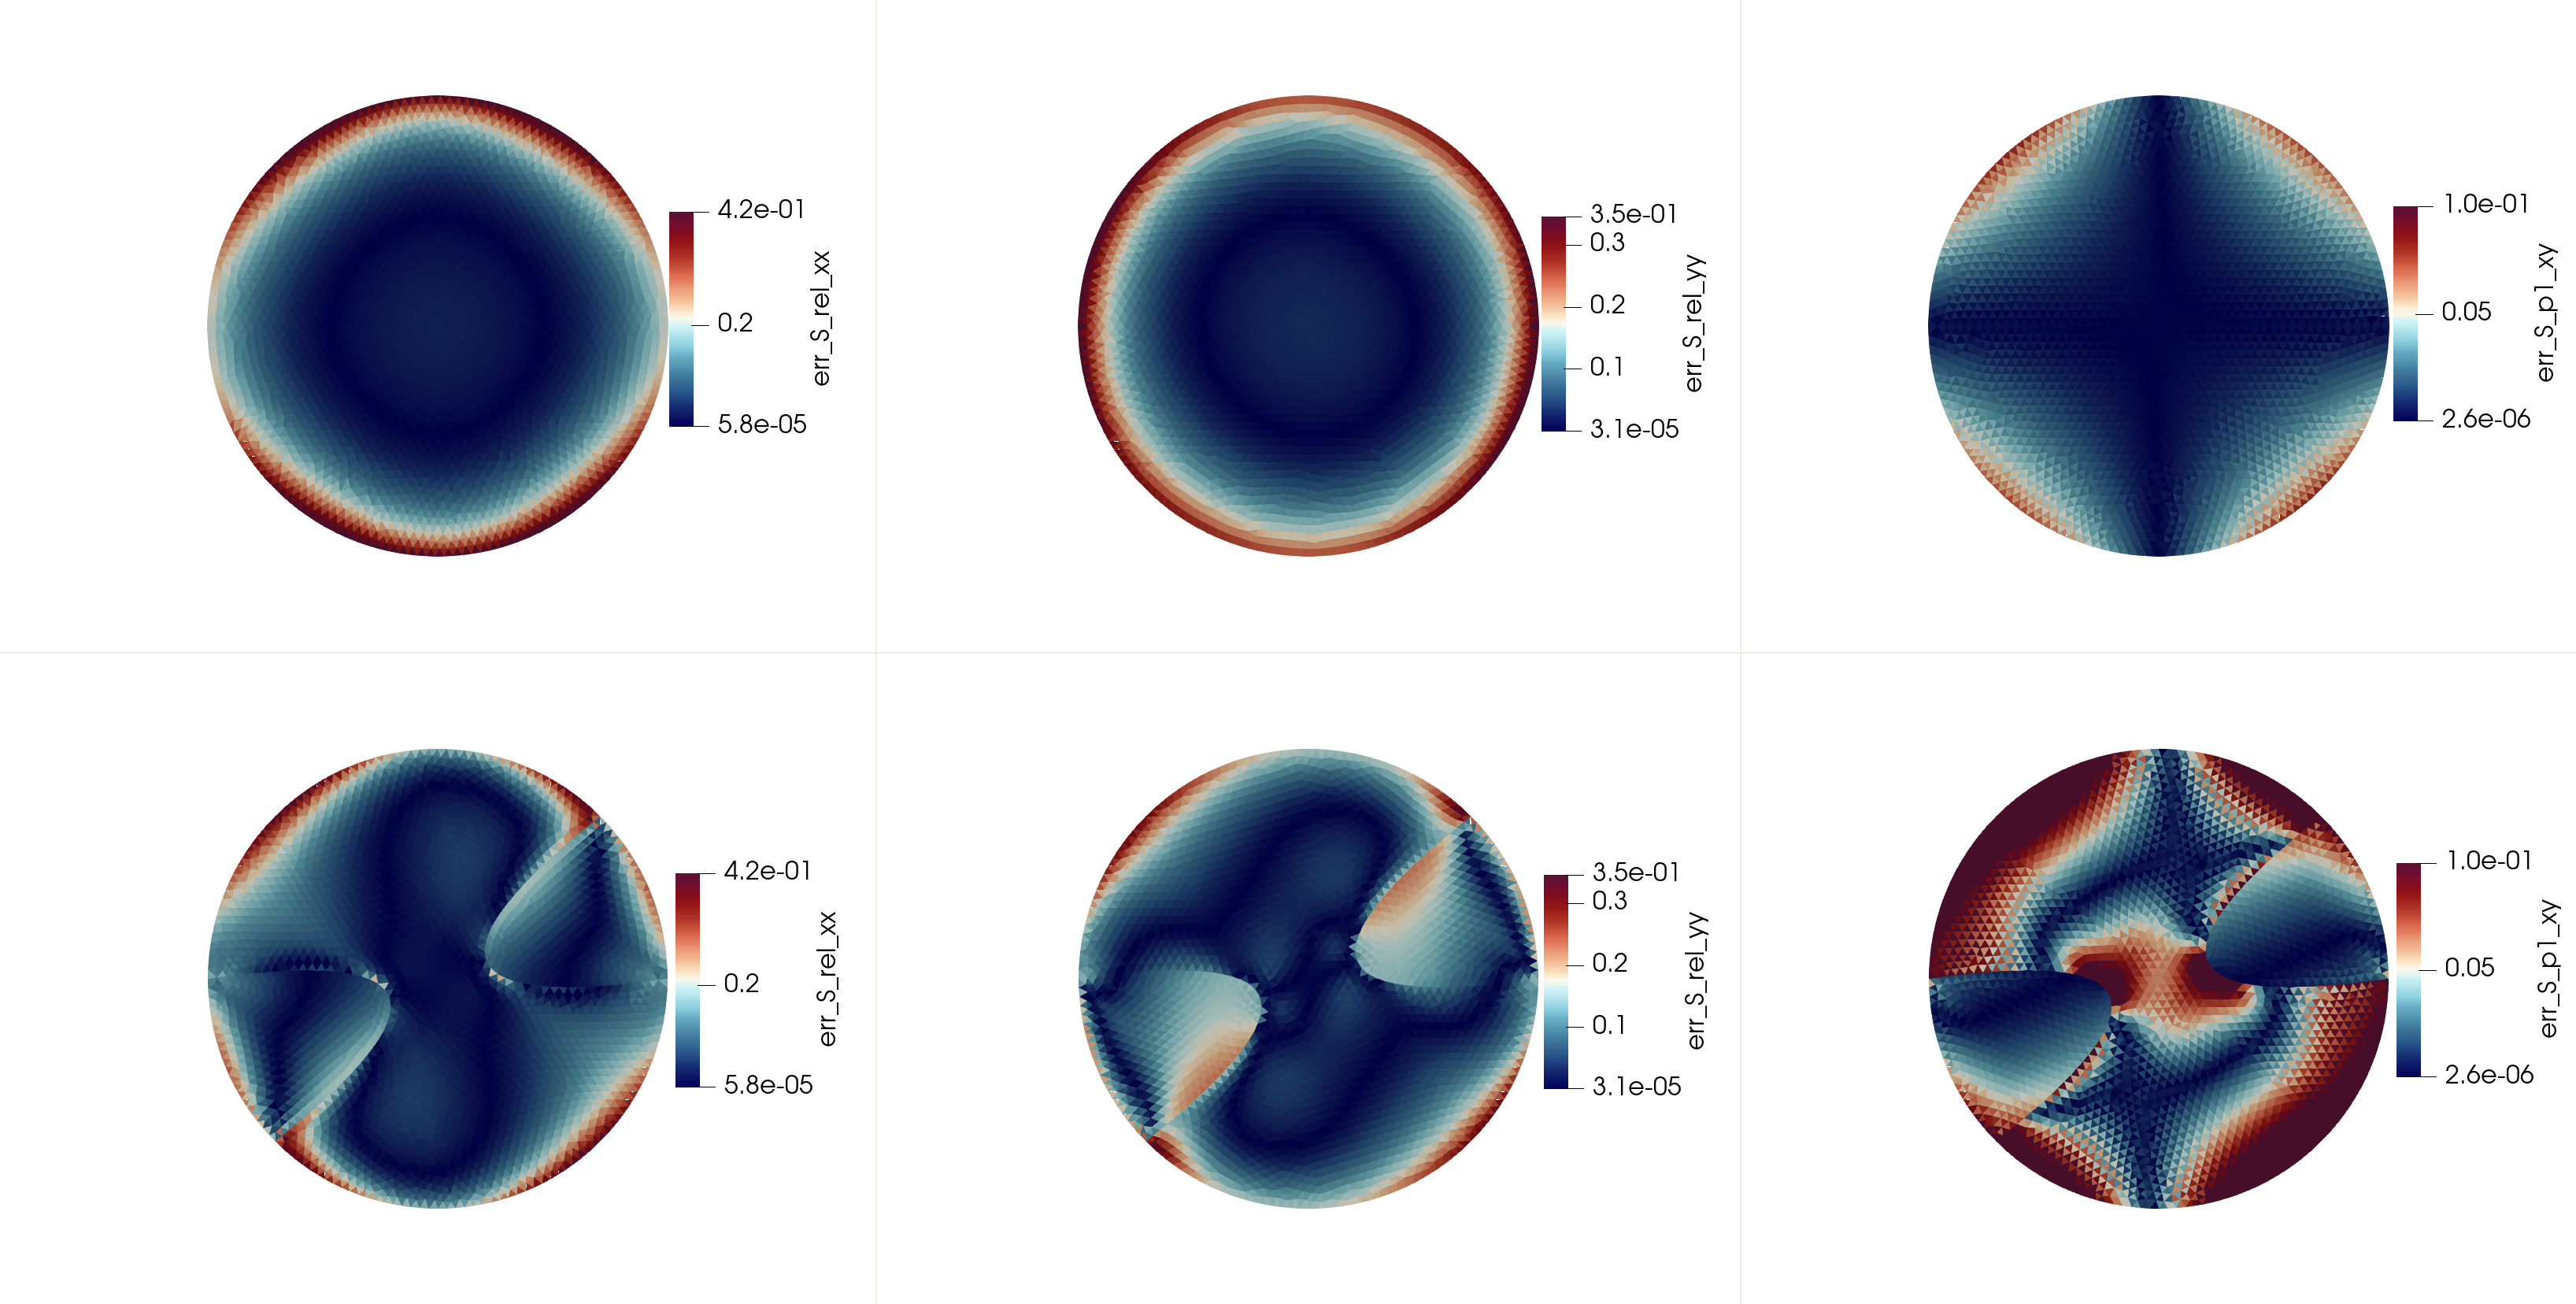
\includegraphics[width=1.0\textwidth]{../img/Numerical/errs.png}
    \caption{Error field between predicted and reference stresses.}
    \label{fig:numerical_errors}
  \end{figure}

  \begin{figure}[H]
    \centering
    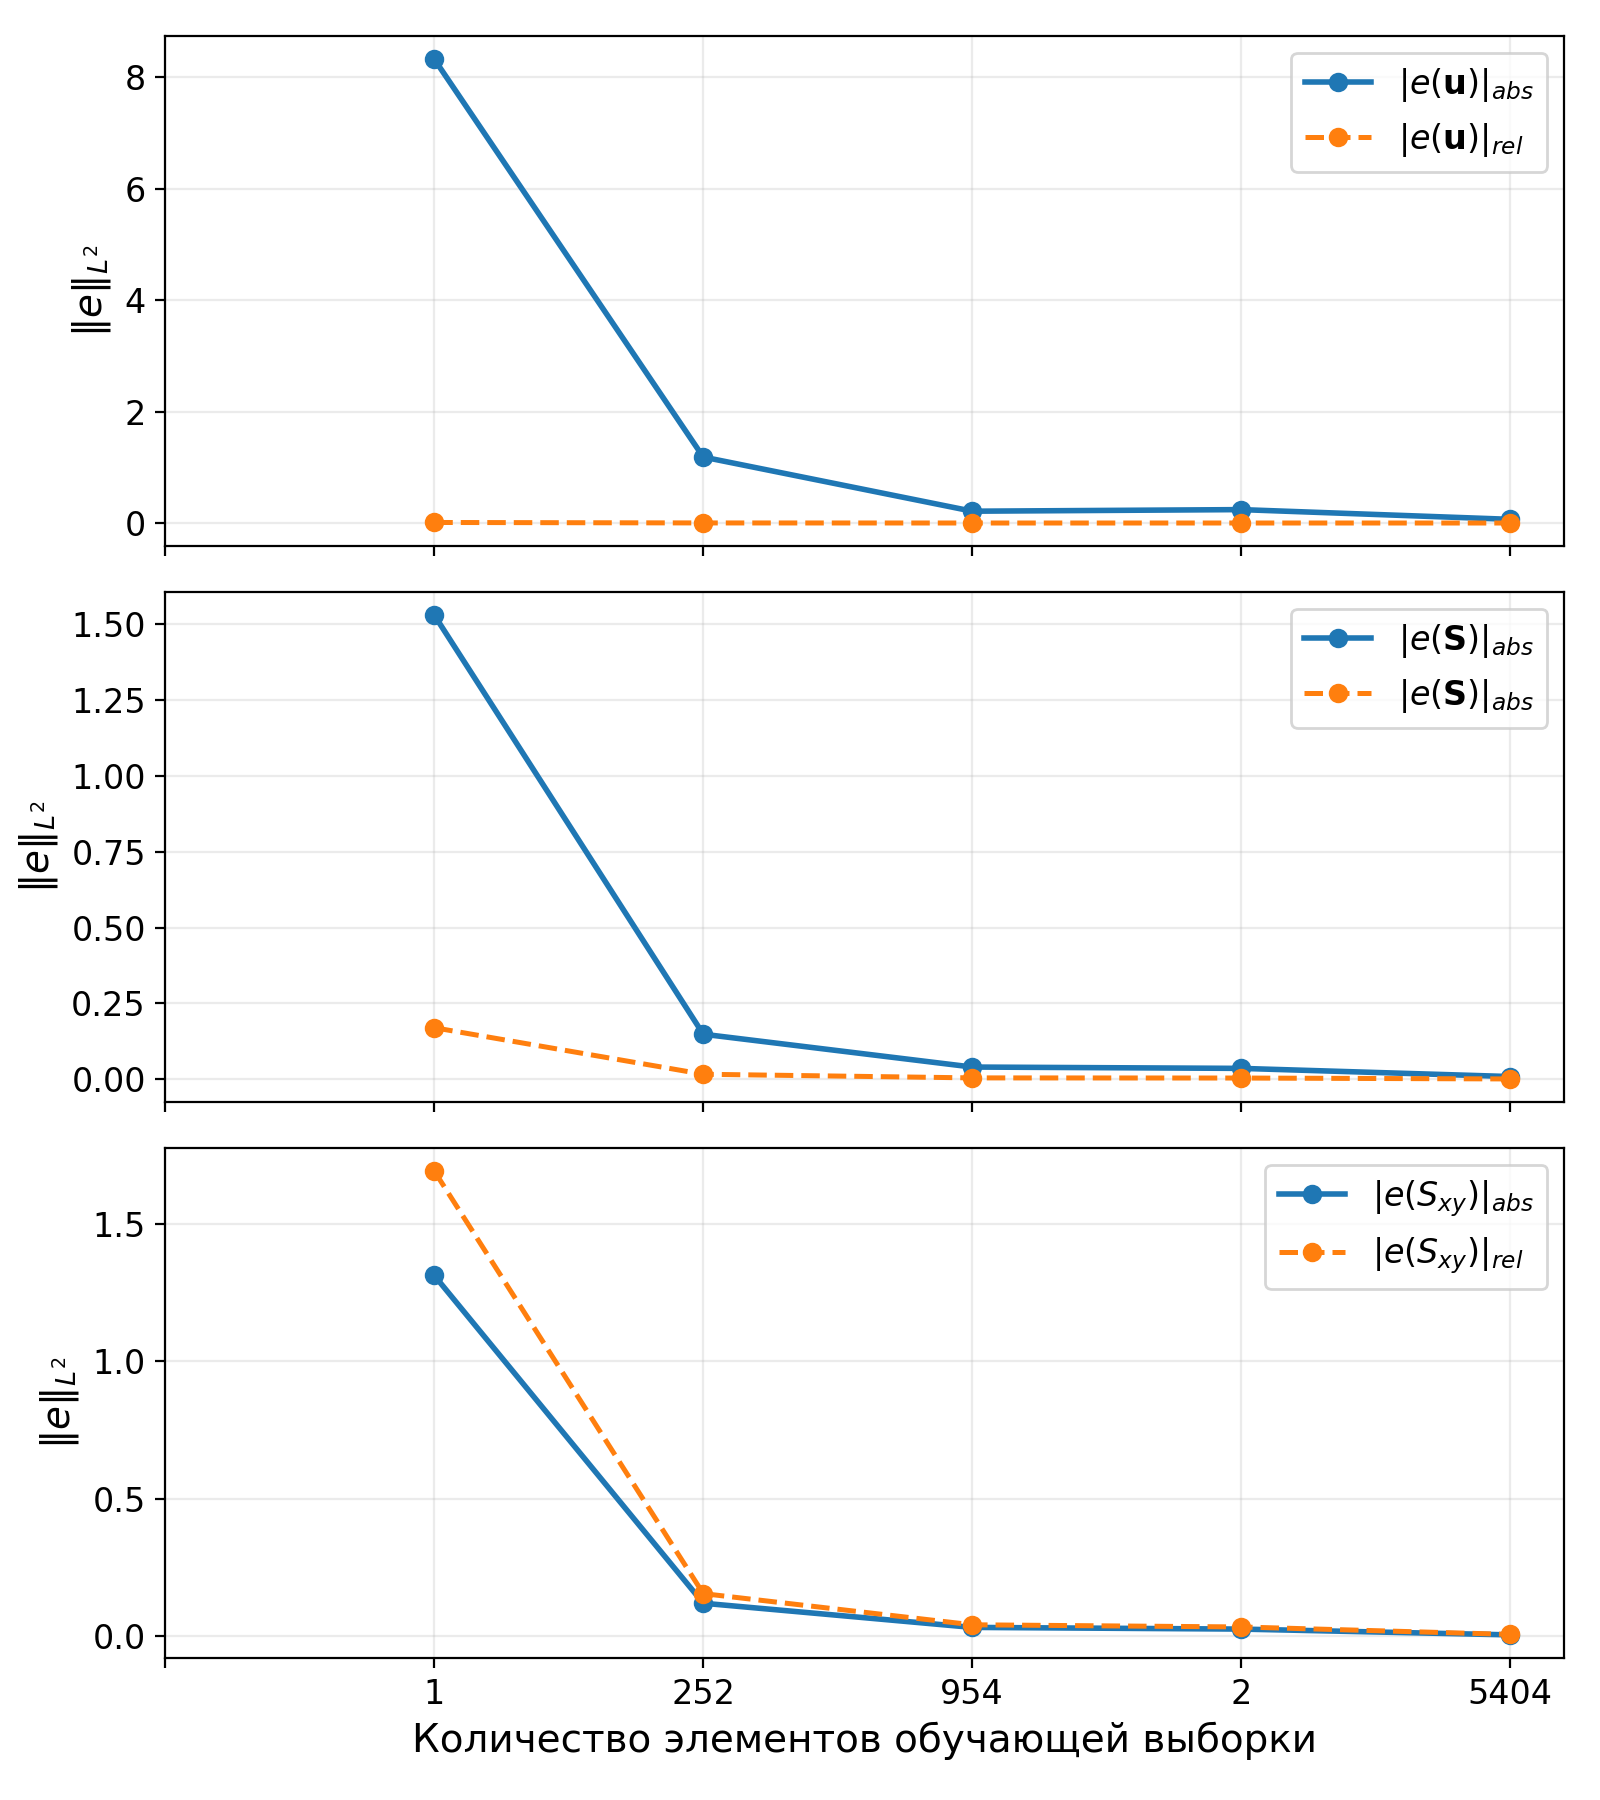
\includegraphics[width=0.5\textwidth]{../img/integral_errors.png}
    \caption{Integral errors $\|e\|_{L^2}$ and $\|e\|_{L^2,\,\mathrm{rel}}$ vs observation-window size $w$.}
    \label{fig:integral_errors}
  \end{figure}
  
  % integral errors vs window (omitted)
  
\subsection{Computational efficiency comparison}

  By strict convexity of $\psi(\boldsymbol\xi)$, the equilibrium is a smooth convex minimization amenable to gradient and Newton-type solvers with predictable complexity \cite{BoydVandenberghe2004,Nesterov2004,NocedalWright2006,ConnGouldToint2000}. Near the minimizer, strong convexity and Lipschitz Hessians yield locally quadratic Newton convergence, while L\textendash BFGS gives superlinear rates \cite{NocedalWright2006}.

  In tabulated/interpolatory DD models (kNN/IDW), energy convexity is typically not guaranteed and responses may be nonsmooth, yielding nonconvex optimization with many stationary points; quasi-static/relaxation strategies are used in practice \cite{KirchdoerferOrtiz2016,KirchdoerferOrtiz2017} at the cost of more load steps/iterations and repeated kNN/IDW queries.

  We compare runtime for CLANN, Neo-Hookean, and a Laplace-space table-driven DD model \cite{xi2023} on inflation of a clamped circular membrane ($R{=}25$ mm), with homogeneous and heterogeneous $T$ (Figure~\ref{fig:membrane_thickness}). CLANN is trained on $D(\{1..10\},\,w{=}\text{1-element})$; the DD model uses kNN/IDW on $(\vect{\xi},\vect r)$ from $D(\{1..10\},\,w{=}10\times10)$ \cite{xi2023}. All runs use the same FE setting and stopping criteria.

\begin{table}[htbp]
\centering
\caption{Runtime (s) for inflation: homogeneous vs heterogeneous thickness}
\label{tab:experiments_summary}
\begin{tabular}{|l|c|c|}
\hline
\textbf{Method} & \textbf{Homogeneous} & \textbf{Heterogeneous} \\
\hline
CLANN & 512 & 329  \\
\hline
Neo-Hooke & 13 & 16\\
\hline
kNN & 993 & -- \\
\hline
\end{tabular}
\end{table}

  With identical meshes and tolerances, CLANN matches Neo-Hooke in global iterations but can be slower overall due to model–solver interface overhead \cite{xi2023}. It notably outperforms the table-driven DD baseline by avoiding repeated kNN/IDW queries and data projections. The DD model further struggles on heterogeneous thickness without linear interpolation near zero, likely due to data scarcity in that strain range.


